\documentclass[tikz,border=12pt]{standalone}
\usepackage{fontspec}
\setmainfont{Segoe UI}
\usepackage{amsmath,amssymb}
\usepackage{tikz}

\usetikzlibrary{calc,arrows.meta}

\begin{document}
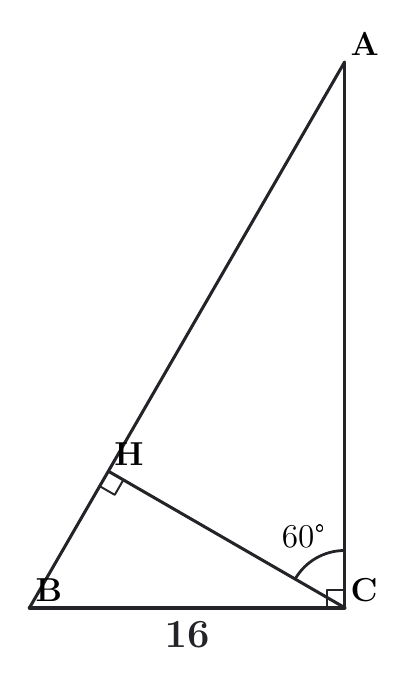
\begin{tikzpicture}[x=1.0000cm,y=1cm,line cap=round,line join=round]
\definecolor{linec0}{RGB}{35,35,40}
\definecolor{linec1}{RGB}{35,35,40}
\definecolor{linec2}{RGB}{35,35,40}
\definecolor{linec3}{RGB}{35,35,40}
\definecolor{linec4}{RGB}{35,35,40}
\definecolor{linec5}{RGB}{35,35,40}
\definecolor{edgecol}{RGB}{35,35,40}
\definecolor{hicol}{RGB}{35,35,40}
\definecolor{angcol}{RGB}{35,35,40}
\coordinate (C) at (0.0000,0.0000);
\coordinate (B) at (-4.0000,0.0000);
\coordinate (A) at (0.0000,6.9282);
\coordinate (H) at (-3.0000,1.7321);
\draw[edgecol,line width=1.1pt] (A) -- (B);
\draw[line width=1.4pt,color={rgb,255:red,35;green,35;blue,40}] (B) -- (C);
\draw[edgecol,line width=1.1pt] (C) -- (A);
\draw[edgecol,line width=1.1pt] (C) -- (H);
\draw[edgecol,line width=0.7pt] (0.000,0.220) -- (-0.220,0.220) -- (-0.220,0.000);
\draw[edgecol,line width=0.7pt] (-2.809,1.622) -- (-2.919,1.432) -- (-3.110,1.542);
\draw[edgecol,line width=1.00pt] (0.000,0.000)++(90.00:0.725) arc[start angle=90.00, delta angle=60.00, radius=0.725];
\node[text=black,font=\large] at (-0.522,0.905) {60°};
\node[font=\bfseries\Large,text={rgb,255:red,35;green,35;blue,40}] at (-2.000,-0.350) {16};
\node[font=\bfseries\large,inner sep=2pt,anchor=south west] at (0.000,0.000) {C};
\node[font=\bfseries\large,inner sep=2pt,anchor=south west] at (-4.000,0.000) {B};
\node[font=\bfseries\large,inner sep=2pt,anchor=south west] at (0.000,6.928) {A};
\node[font=\bfseries\large,inner sep=2pt,anchor=south west] at (-3.000,1.732) {H};
\end{tikzpicture}
\end{document}
